\chapter{Interfacing a Pushbutton}
\thispagestyle{empty}
\label{pushbutton}

\newcommand{\LocPushfig}{\Origin/user-code/push/figures}
\newcommand{\LocPushscicode}{\Origin/user-code/push/scilab}
\newcommand{\LocPushscibrief}[1]{{\tt
    \seqsplit{Origin/user-code/push/scilab/#1}}, 
see \fnrefp{fn:file-loc}}
\newcommand{\LocPushardcode}{\Origin/user-code/push/arduino}
\newcommand{\LocPushardbrief}[1]{{\tt
    \seqsplit{Origin/user-code/push/arduino/#1}}, 
see \fnrefp{fn:file-loc}}


%%%%%%%%%%%%%%python starts
\newcommand{\LocPushpycode}{\Origin/user-code/push/python}
\newcommand{\LocPushpybrief}[1]{{\tt
    \seqsplit{Origin/user-code/push/python/#1}}, 
see \fnrefp{fn:file-loc}}
%%%%%%%%%%%%%python ends

%%%%%%%%%%%%%%julia starts
\newcommand{\LocPushjuliacode}{\Origin/user-code/push/julia}
\newcommand{\LocPushjuliabrief}[1]{{\tt
    \seqsplit{Origin/user-code/push/julia/#1}}, 
see \fnrefp{fn:file-loc}}
%%%%%%%%%%%%%julia ends


%%%%%OpenModelica starts
\newcommand{\LocPushOpenModelicacode}{\Origin/user-code/push/OpenModelica}  %added for OpenModelica
\newcommand{\LocPushOpenModelicabrief}[1]{{\tt \seqsplit{%
    Origin/user-code/led/OpenModelica/#1}}, see \fnrefp{fn:file-loc}} % added for OpenModelica
%%%%%%OpenModelica Ends

A pushbutton is a simple switch which is used to connect or disconnect
a circuit. It is commonly available as a \emph{normally open} or
\emph{push to make} switch which implies that the contact is made upon
the push or depression of the switch. These switches are widely used
in calculators, computer keyboards, home appliances, push-button
telephones and basic mobile phones, etc. In this chapter, we shall
perform an experiment to read the status of the pushbutton mounted
on the shield of the \arduino\ board. Advancing further, we shall
perform a task depending on the status of the pushbutton. Digital
logic based status monitoring is a very basic and important task in
many industrial applications. This chapter will enable us to have a
smooth hands-on for such functionalities. 

\section{Preliminaries}
A pushbutton mounted on the shield is connected to the digital pin 12
of the \arduino\ board. The connection diagram for the pushbutton is
shown in \figref{fig:pushbuttonconn}. It has 2 pairs of
terminals. Each pair is electrically connected. When the pushbutton is
pressed all the terminals short to complete the circuit, thereby
allowing the flow of current through the switch. As you might expect,
there is a limit to the maximum current that could flow through a
pushbutton. This maximum current is also called the rated current and
is usually provided by the manufacturer in the datasheet.  

\begin{figure}
\centering
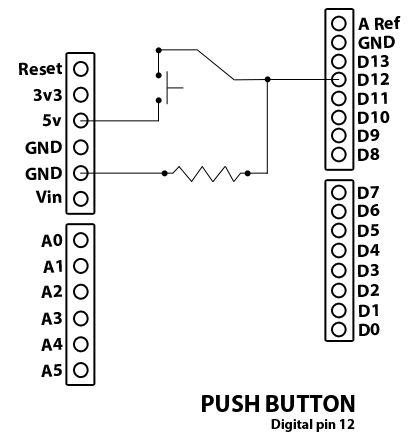
\includegraphics[width=\smfig]{\LocPushfig/pushbutton-conn.png}
\caption{Connection Diagram}
%\redcolor{connected on pin no. D12}}
\label{fig:pushbuttonconn}
\end{figure}


\begin{figure}
  \centering
  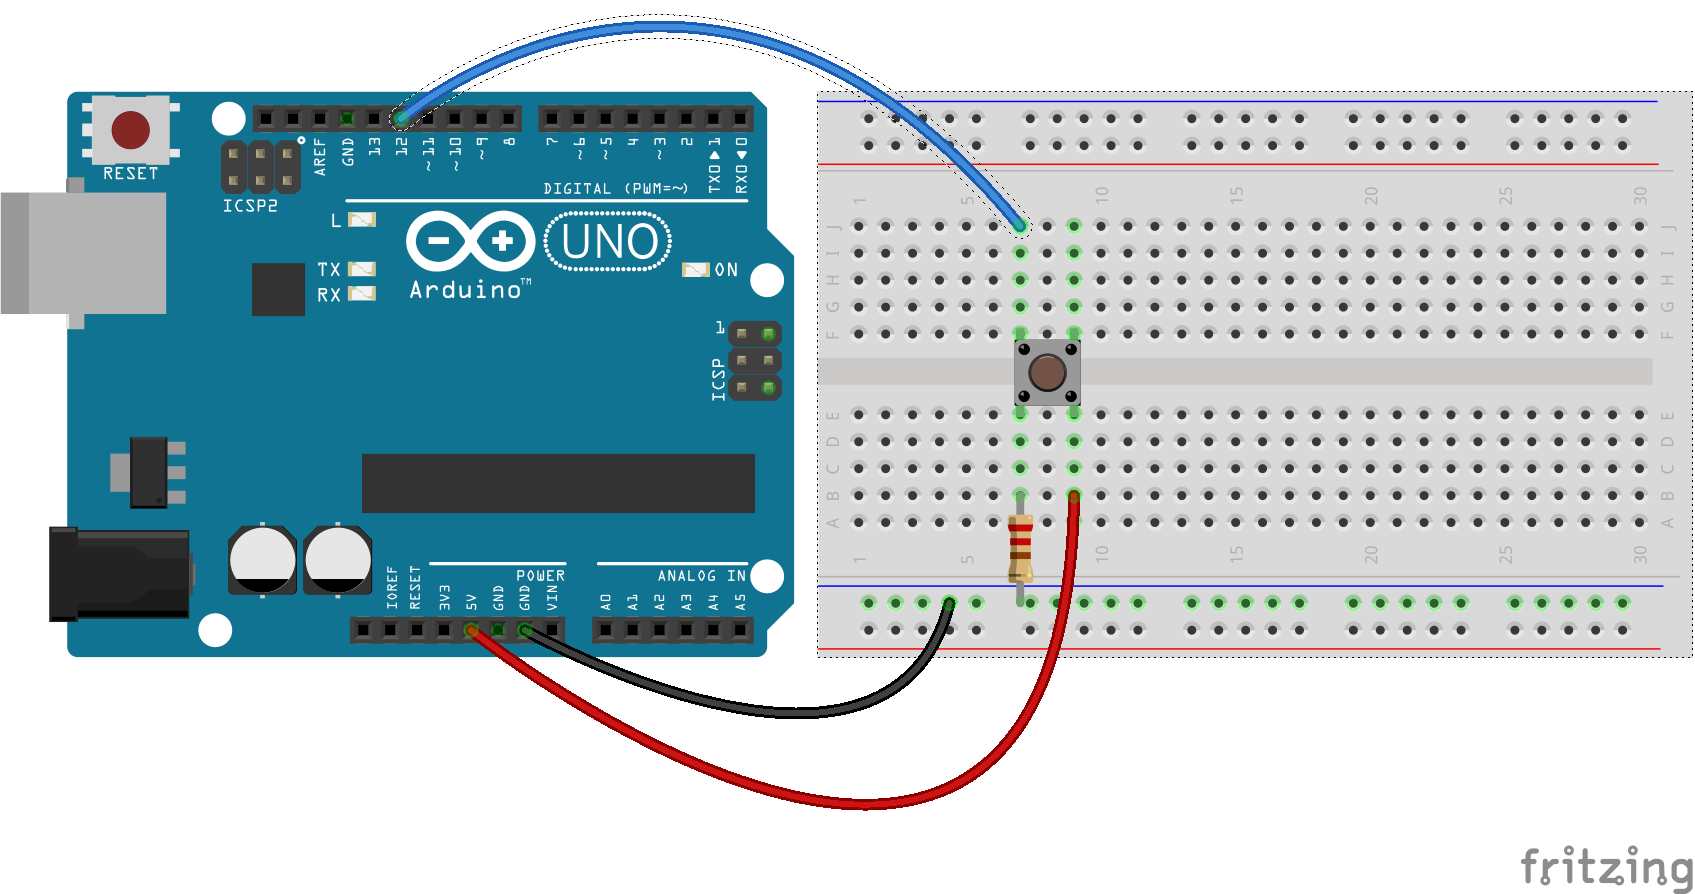
\includegraphics[width=\textwidth]{\LocPushfig/switch.png}
  \caption{A pushbutton to read its status with Arduino Uno using a breadboard}
  %\redcolor{connected on pin no. D12}}
  \label{fig:switch-bread}
\end{figure}

\section{Connecting a pushbutton with \arduino\ using a breadboard}
This section is useful for those who either don't have a shield or don't want to use the shield
for performing the experiments given in this chapter. 

A breadboard is a device for holding the components of a circuit and connecting 
them together. We can build an electronic circuit on a breadboard without doing any 
soldering. To know more about the breadboard and other electronic components, 
one should watch the Spoken Tutorials on Arduino as published on
{\tt https://spoken-tutorial.org/}. Ideally, one should go through all the
tutorials labeled as Basic. However, we strongly recommend the readers should
watch the fifth and sixth tutorials, i.e., {\tt First Arduino Program} and 
{\tt Arduino with Tricolor LED and Push button}.

In case you have a pushbutton, and you want to connect it with \arduino\ on a breadboard, 
please refer to \figref{fig:switch-bread}. The connections given in this figure can be used to 
read the status of a pushbutton. As shown in \figref{fig:switch-bread}, 
there are three different wires - red, black, and blue. The red wire is used to connect 5V on 
\arduino\ and one leg of the pushbutton. The black wire connects to one long vertical row on 
the side of the breadboard to provide access to the ground (GND) on \arduino. 
The blue wire goes from digital pin 12 to one leg of the pushbutton on another side. 
That same leg of the pushbutton connects through a pull-down resistor to GND on \arduino. 
When the pushbutton is open (unpressed), there is no connection between the two legs of the pushbutton, 
so the pin is connected to the ground (through the pull-down resistor), and we read a LOW on
digital pin 12. When the pushbutton is closed (pressed), it makes a connection between its two legs, 
connecting the pin to 5V so that we read a HIGH on digital pin 12. 

\begin{figure}
  \centering
  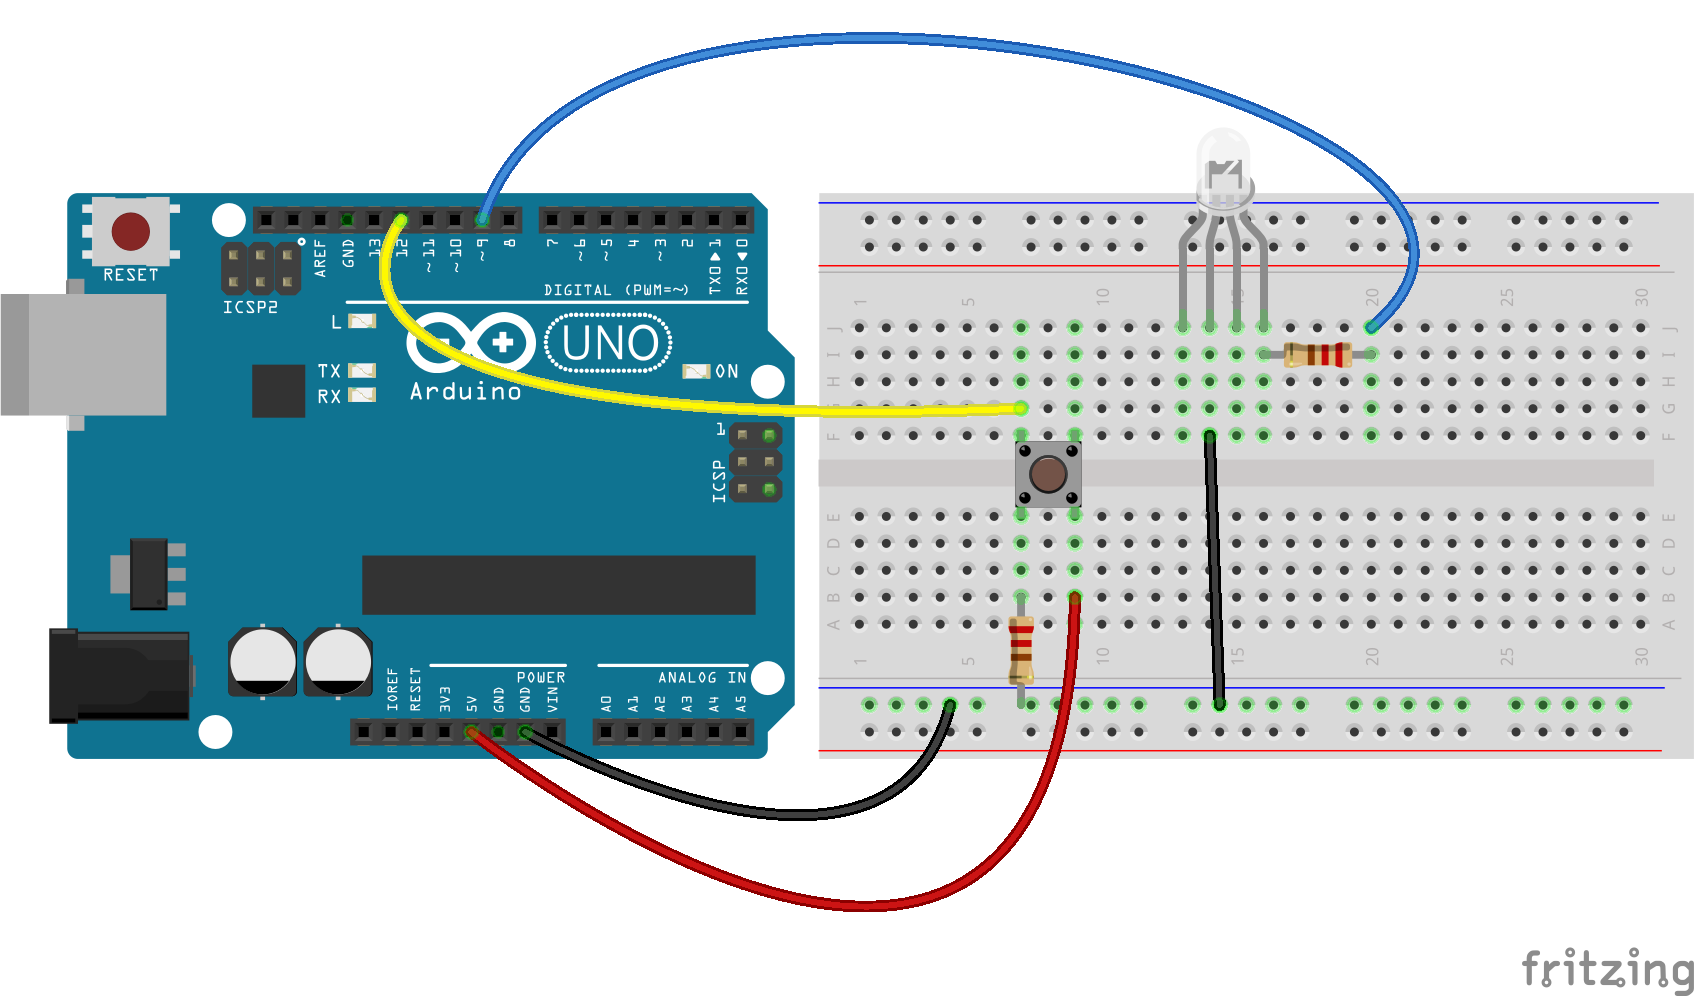
\includegraphics[width=\textwidth]{\LocPushfig/switch-led.png}
  \caption{A pushbutton to control an LED with Arduino Uno using a breadboard}
  %\redcolor{connected on pin no. D12}}
  \label{fig:switch-led}
\end{figure}
The connections shown in \figref{fig:switch-led} can be used to control an RGB LED, 
depending on the status of the pushbutton. As shown in \figref{fig:switch-led}, digital
pin 9 on \arduino\ is connected to the rightmost leg of the RGB LED. Rest of the connections
are same as that in \figref{fig:switch-bread}. 

\section{Reading the Pushbutton Status from the Arduino IDE}
\subsection{Reading the Pushbutton Status}
In this section, we shall describe an experiment that will help 
to read the status of a pushbutton through Arduino IDE. 
Later, we shall change the state of an LED depending on the status of the pushbutton. The shield has to be attached to the \arduino\ board
before doing these experiments and the \arduino\ needs to be connected to the computer 
with a USB cable, as shown in \figref{arduino}. The reader should go through the
instructions given in \secref{sec:ard-start} before getting started.
\begin{enumerate}
\item In the first experiment, we shall simply read the status of the
  pushbutton. Recall that it is a normally open type of switch. So, in
  an unpressed state, the logic read will be ``0'', corresponding to
  0V. And, when the user presses the pushbutton, the reading would be
  ``1'', corresponding to 5V. The code for this experiment is given in
  \ardref{ard:push-100}. In the initialization part of the code, we
  assign the sensor pin to be read, 12 in this case, to a variable for
  ease. Next, we initialize the port for serial port communication at
  data rate of 115200 bits per second and declare the digital pin 12 as an 
  input pin using the command {\tt pinMode}.  After initialization, 
  we start reading the status of the pushbutton using the following command:
  \lstinputlisting[firstline=7,lastline=7]
  {\LocPushardcode/push-button-status/push-button-status.ino}

  Note that the input argument to this command is the digital pin 12
  corresponding to the pin to which the pushbutton is connected.  After
  acquiring the values, we print them using,
  \lstinputlisting[firstline=8,lastline=8]
  {\LocPushardcode/push-button-status/push-button-status.ino} We
  repeat this read and print process 1000 times by putting the
  commands in a {\tt for} loop. While running this experiment, the readers must press
  and release the pushbutton and observe the values being printed on the
  {\tt Serial Monitor} of Arduino IDE.

\item In the second experiment, we shall control the power given to an
  LED as per the status of the pushbutton. The code for this
  experiment is given in \ardref{ard:push-200}. This experiment can be
  taken as a step further to the previous one. We declare the LED pin
  to be controlled as an output pin by,
  \lstinputlisting[firstline=7,lastline=7]
  {\LocPushardcode/led-push-button/led-push-button.ino} Next, we read
  the pusbhutton value from digital pin 12. If the value is ``1'',
  we turn on the LED at pin 9 else we turn it off. The
  condition check is performed using {\tt if else} statements. We run
  these commands for 1000 iterations. While running this experiment, the readers 
  must press and release the pushbutton. Accordingly, they can observe whether 
  the LED glows when the pushbutton is pressed. 
  %  \redcolor{Serial monitor}.
\end{enumerate}

\subsection{Arduino Code}
\lstset{style=mystyle}
\label{sec:push-arduino-code}
\addtocontents{ard}{\protect\addvspace{\codclr}}

\begin{ardcode}
  \acaption{Read the status of the pushbutton and display it on the
  Serial Monitor}{Read the status of the pushbutton and display it on
    the Serial Monitor.  Available at
    \LocPushardbrief{push-button-status/push-button-status.ino}.}
\label{ard:push-100}
\lstinputlisting{\LocPushardcode/push-button-status/push-button-status.ino}
\end{ardcode}

\begin{ardcode}
  \acaption{Turning the LED on or off depending on the pushbutton}
  {Turning the LED on or off depending on the pushbutton.  Available
    at \LocPushardbrief{led-push-button/led-push-button.ino}.}
\label{ard:push-200}
\lstinputlisting{\LocPushardcode/led-push-button/led-push-button.ino}
\end{ardcode}


\section{Reading the Pushbutton Status from Scilab}
\subsection{Reading the Pushbutton Status}
In this section, we discuss how to carry out the experiments of the
previous section from Scilab. We will list the same two experiments,
in the same order.  The shield has to be attached to the \arduino\ board
before doing these experiments and the \arduino\ needs to be connected to the computer 
with a USB cable, as shown in \figref{arduino}.
The reader should go through the instructions given in
\secref{sec:sci-start} before getting started. 
\begin{enumerate}
\item In the first experiment, we will read the pushbutton status using a 
Graphical user interface (GUI) in Scilab. The code for this experiment is 
given in  \sciref{sci:push-100}. As explained earlier in \secref{sec:light-sci}, 
we begin with serial port initialization. Then, we read the input coming from
digital pin 12 using the following command: 
  \lstinputlisting[firstline=4,lastline=4]
  {\LocPushscicode/push-button-status.sce} Note that the one leg of the pushbutton on
  the shield is connected to digital pin 12 of \arduino\, 
  as given in \figref{fig:pushbuttonconn}. The read value is displayed as a GUI using
  the following command: \lstinputlisting[firstline=5,lastline=5]
  {\LocPushscicode/push-button-status.sce} where {\tt val} contains
  the pushbutton value acquired by the previous command.
  When the pushbutton is not pressed, {\tt val} will be ``0''. On the other hand,
  when the pushbutton is pressed, {\tt val} will be ``1''. To
  encourage the user to have a good hands-on, we run these commands in
  a {\tt for} loop for 1000 iterations. While running this experiment, 
  the readers must press and release the pushbutton and observe the values being printed on the
  GUI, as shown in \figref{fig:ard-meter}.
 \begin{figure}
    \centering
    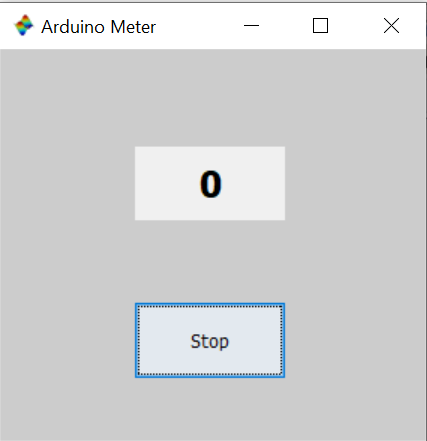
\includegraphics[width=\smfig]{\LocPushfig/sci-ard-meter.png}
    \caption{GUI in Scilab to show the status of the pushbutton}
    %\redcolor{connected on pin no. D12}}
    \label{fig:ard-meter}
  \end{figure}
\item This experiment is an extension of the previous
  experiment. Here, we control the state of an LED as per the status
  of the pushbutton. In other words, digital output to an LED is
  decided by the digital input received from the pushbutton. The code
  for this experiment is given in \sciref{sci:push-200}. After reading
  the pushbutton status, we turn the LED on if the pushbutton is
  pressed, otherwise we turn it off. The following lines,
  \lstinputlisting[firstline=5,lastline=9]
  {\LocPushscicode/led-push-button.sce} perform the condition check
  and corresponding LED state control operation. While running this experiment, the readers 
  must press and release the pushbutton. Accordingly, they can observe whether 
  the LED glows when the pushbutton is pressed. 
\end{enumerate}

\subsection{Scilab Code}
\label{sec:push-scilab-code}
\addtocontents{cod}{\protect\addvspace{\codclr}}

\begin{scicode}
\ccaption{Read the status of the pushbutton and display it on the GUI}
{Read the status of the pushbutton and display it on the GUI.  Available at
  \LocPushscibrief{push-button-status.sce}.}
\label{sci:push-100}
\lstinputlisting{\LocPushscicode/push-button-status.sce}
\end{scicode}

\begin{scicode}
\ccaption{Turning the LED on or off depending on the pushbutton}
  {Turning the LED on or off depending on the pushbutton.  Available at
  \LocPushscibrief{led-push-button.sce}.}
\label{sci:push-200}
\lstinputlisting{\LocPushscicode/led-push-button.sce}
\end{scicode}




\section{Accessing the Pushbutton from Xcos}
\label{sec:push-xcos}
In this section, we will see how to access the pushbutton from Scilab
Xcos.  We will carry out the same two experiments as in the previous
sections.  For each, will give the location of the zcos file and the
parameters to set.  The reader should go through the instructions
given in \secref{sec:xcos-start} before getting started.

\begin{enumerate}
\item First we will read the push button value and print it.  When the
  file required for this experiment is invoked, one gets the GUI as in
  \figref{fig:push-button-status}.  In the caption of this figure, one
  can see where to locate the file.

  As discussed in earlier chapters, we start with the initialization
  of the serial port. Next, using {\tt Digital Read} block, we read
  the status of pushbutton connected on digital pin 12. The read
  values are displayed.  When a user presses the pushbutton, change in
  the logic value from low to high can be observed.

  \begin{figure}
    \centering
    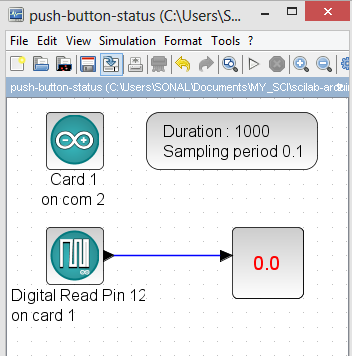
\includegraphics[width=\smfig]{\LocPushfig/push-button-status.PNG}
    \caption[Printing the push button status on the display block]
    {Printing the push button status on the display block.  This is
      what one sees when
        \LocPushscibrief{push-button-status.zcos}, is invoked.}
    \label{fig:push-button-status}
  \end{figure}

  We will next explain how to set the parameters for this simulation.
  To set value on any block, one needs to right click and open the
  {\tt Block Parameters} or double click.  The values for each block
  is tabulated in \tabref{tab:push-button-status}.  All other
  parameters are to be left unchanged.
  \begin{table}
    \centering
    \caption{Parameters to print the push button status on the display
      block} 
    \label{tab:push-button-status}
    \begin{tabular}{llc} \hline
      Name of the block & Parameter name & Value \\ \hline
      ARDUINO\_SETUP & Identifier of Arduino Card & 1 \\
      & Serial com port number & 2\portcmd \\ \hline
      TIME\_SAMPLE & Duration of acquisition(s) & 10 \\
      & Sampling period(s) & 0.1 \\ \hline
      DIGITAL\_READ\_SB & Digital pin & 12 \\
      & Arduino card number & 1 \\ \hline 
      AFFICH\_m & Block inherits (1) or not  (0) & 1 \\ \hline
    \end{tabular}
  \end{table}

\item In the second experiment, we take a step further and control the
  state of an LED in accordance with the status of the pushbutton. The
  Xcos implementation for this experiment is shown in
  \figref{fig:led-push-button}. Each time a user presses the
  pushbutton, the LED on digital pin 9 of the shield is switched
  on. If the shield is connected, the blue LED turns on.  When
  the pushbutton is released, the LED is switched off. Here, we note that
  the digital logic level of the pin of the \arduino\ board connected
  to pushbutton changes only for the time the pushbutton is being
  pressed.

  \begin{figure}
    \centering
    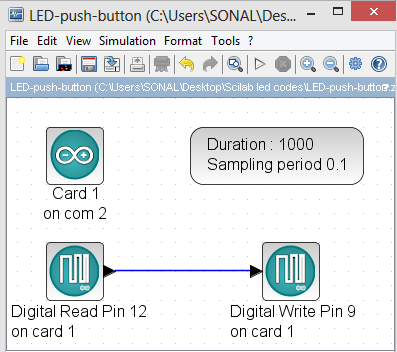
\includegraphics[width=\smfig]{\LocPushfig/led-push-button.PNG}
    \caption[Turning the LED on or off, depending on the pushbutton]
    {Turning the LED on or off, depending on the pushbutton.  This is
      what one sees when
        \LocPushscibrief{led-push-button.zcos}, is invoked.}
    \label{fig:led-push-button}
  \end{figure}

  We will next explain how to set the parameters for this simulation.
  To set value on any block, one needs to right click and open the
  {\tt Block Parameters} or double click.  The values for each block
  is tabulated in \tabref{tab:led-push-button}.  All other
  parameters are to be left unchanged.
  \begin{table}
    \centering
    \caption{Xcos parameters to turn the LED on through the pushbutton}
    \label{tab:led-push-button}
    \begin{tabular}{llc} \hline
      Name of the block & Parameter name & Value \\ \hline
      ARDUINO\_SETUP & Identifier of Arduino Card & 1 \\
      & Serial com port number & 2\portcmd \\ \hline
      TIME\_SAMPLE & Duration of acquisition(s) & 10 \\
      & Sampling period(s) & 0.1 \\ \hline
      DIGITAL\_READ\_SB & Digital pin & 12 \\
      & Arduino card number & 1 \\ \hline 
      DIGITAL\_WRITE\_SB & Digital pin & 9 \\
      & Card number & 1 \\ \hline
    \end{tabular}
  \end{table}
\end{enumerate}

\begin{exercise}
Let us carry out the following exercise:
\begin{enumerate}
\item In the above experiment, we controlled only one LED upon
  pushbutton press. Next, control multiple devices upon the pushbutton
  press. For example, upon press, turn on an LED and a motor and turn
  them off upon release.
\item Control several devices depending on the number of pushbutton
  press in a definite time span. For example, if the pushbutton is
  pressed once in time 't',say, turn on the LED. If it is pressed
  twice in time 't', turn on the motor. Here, you may want to consider
  the timing between two consecutive press.
\end{enumerate}
\end{exercise}

%%%%%%%%%%%%python description starts
\section{Reading the Pushbutton Status from Python}
\subsection{Reading the Pushbutton Status}
In this section, we discuss how to carry out the experiments of the
previous section from Python.  We will list the same two experiments,
in the same order.  The shield has to be attached to the \arduino\ board
before doing these experiments and the \arduino\ needs to be connected to the computer 
with a USB cable, as shown in \figref{arduino}.
The reader should go through the instructions given in
\secref{sec:python-start} before getting started.

\begin{enumerate}
\item In the first experiment, we will read the pushbutton status. The code for this experiment is given in
  \pyref{py:push-100}. As explained earlier in \secref{sec:light-py}, we begin with 
  importing necessary modules followed by setting up the serial port. 
  Then, we read the input coming from digital pin 12 using the
  following command:
  \lstinputlisting[firstline=26,lastline=26]
  {\LocPushpycode/push-button-status.py} Note that the one leg of the pushbutton on
  the shield is connected to digital pin 12 of \arduino\, 
  as given in \figref{fig:pushbuttonconn}. The read value is displayed (or printed) 
 by the following lines: 
   \lstinputlisting[firstline=25,lastline=28]
  {\LocPushpycode/push-button-status.py} where {\tt val} contains
  the pushbutton value acquired by the previous command. When the pushbutton is not pressed, {\tt val} will be ``0''. On the other hand,
  when the pushbutton is pressed, {\tt val} will be ``1''.
  To encourage the user to have a good hands-on, we run these commands in
  a {\tt for} loop for 20 iterations. The readers are encouraged to change the number 
  of iterations as per their requirements. While running this experiment, the readers must press
  and release the pushbutton and observe the values being printed on the
  Command Prompt (on Windows) or Terminal (on Linux), as the case maybe.


\item This experiment is an extension of the previous
  experiment. Here, we control the state of an LED as per the status
  of the pushbutton. In other words, digital output to an LED is
  decided by the digital input received from the pushbutton. The code
  for this experiment is given in \pyref{py:push-200}. After reading
  the pushbutton status, we turn the LED on if the pushbutton is
  pressed, otherwise we turn it off. The following lines,
  \lstinputlisting[firstline=28,lastline=33]
  {\LocPushpycode/led-push-button.py} perform the condition check
  and corresponding LED state control operation. While running this experiment, the readers must press and release the push-
  button. Accordingly, they can observe whether the LED glows when the push-
  button is pressed.
\end{enumerate}

\subsection{Python Code}
\lstset{style=mystyle}
\label{sec:push-python-code}
\addtocontents{pyd}{\protect\addvspace{\codclr}}

\begin{pycode}
\pcaption{Read the status of the pushbutton and display it on the
  Command Prompt or the Terminal}{Read the status of the pushbutton and display it on
  Command Prompt or the Terminal.  Available at
  \LocPushpybrief{push-button-status.py}.}
\label{py:push-100}
\lstinputlisting{\LocPushpycode/push-button-status.py}
\end{pycode}

\begin{pycode}
\pcaption{Turning the LED on or off depending on the pushbutton}
  {Turning the LED on or off depending on the pushbutton.  Available at
  \LocPushpybrief{led-push-button.py}.}
\label{py:push-200}
\lstinputlisting{\LocPushpycode/led-push-button.py}
\end{pycode}


\section{Reading the Pushbutton Status from Julia}
\subsection{Reading the Pushbutton Status} 
In this section, we discuss how to carry out the experiments of the
previous section from Julia.  We will list the same two experiments,
in the same order.  The shield has to be attached to the \arduino\ board
before doing these experiments and the \arduino\ needs to be connected to the computer 
with a USB cable, as shown in \figref{arduino}.
The reader should go through the instructions given in \secref{sec:julia-start} before getting started.

\begin{enumerate}
\item In the first experiment, we will read the pushbutton status. 
The code for this experiment is given in \juliaref{julia:push-100}. 
As explained earlier in \secref{sec:light-julia}, we begin with importing the SerialPorts 
\cite{julia-serial-ports} package and the module ArduinoTools followed by setting up the serial port.
Then, we read the input coming from digital pin 12 using the following
command: 
\lstinputlisting[firstline=7,lastline=7]
  {\LocPushjuliacode/push-button-status.jl}
  Note that the one leg of the pushbutton on the shield is connected to digital
pin 12 of Arduino Uno as given in \figref{fig:pushbuttonconn}. The read value is displayed (or
printed) by the following lines:
\lstinputlisting[firstline=6,lastline=8]
  {\LocPushjuliacode/push-button-status.jl} where {\tt val} contains the pushbutton value acquired by the previous command.
  When the pushbutton is not pressed, {\tt val} will be ``0''. On the other hand,
  when the pushbutton is pressed, {\tt val} will be ``1''. To encourage the user to have a good hands-on, we run these commands in a
{\tt for} loop for 200 iterations. The readers are encouraged to change the number
of iterations as per their requirements. While running this experiment, the readers
must press and release the pushbutton and observe the values being printed
on the Command Prompt (on Windows) or Terminal (on Linux), as the case
maybe.

\item This experiment is an extension of the previous
  experiment. Here, we control the state of an LED as per the status
  of the pushbutton. In other words, digital output to an LED is
  decided by the digital input received from the pushbutton. The code
  for this experiment is given in \juliaref{julia:push-200}. After reading
  the pushbutton status, we turn the LED on if the pushbutton is
  pressed, otherwise we turn it off. The following lines, 
  \lstinputlisting[firstline=7,lastline=12]
  {\LocPushjuliacode/led-push-button.jl} perform the condition check
  and corresponding LED state control operation. While running this experiment, the readers must press and release the push-
  button. Accordingly, they can observe whether the LED glows when the push-
  button is pressed.
\end{enumerate}

\subsection{Julia Code}
\label{sec:push-julia-code}
\addtocontents{juliad}{\protect\addvspace{\codclr}}

\begin{juliacode}
\jcaption{Read the status of the pushbutton and display it on Command Prompt or the Terminal.}{Read the status of the pushbutton and display it on Command Prompt or the Terminal.  Available at
  \LocPushjuliabrief{push-button-status.jl}.}
\label{julia:push-100}
\lstinputlisting{\LocPushjuliacode/push-button-status.jl}
\end{juliacode}

\begin{juliacode}
\jcaption{Turning the LED on or off depending on the pushbutton}
  {Turning the LED on or off depending on the pushbutton.  Available at
  \LocPushjuliabrief{led-push-button.jl}.}
\label{julia:push-200}
\lstinputlisting{\LocPushjuliacode/led-push-button.jl}
\end{juliacode}

\section{Reading the Pushbutton Status from OpenModelica}
\subsection{Reading the Pushbutton Status}
In this section, we discuss how to carry out the experiments of the
previous section from OpenModelica.  We will list the same two experiments,
in the same order.  The shield has to be attached to the \arduino\ board
before doing these experiments and the \arduino\ needs to be connected to the computer 
with a USB cable, as shown in \figref{arduino}.
The reader should go through the instructions given in
\secref{sec:OpenModelica-start} before getting started.

\begin{enumerate}
\item In the first experiment, we will read the pushbutton status. The code for this experiment is given in
  \OpenModelicaref{OpenModelica:push-100}. As explained earlier in \secref{sec:light-OpenModelica}, 
  we begin with importing the two packages: Streams and SerialCommunication followed 
  by setting up the serial port. Then, we read the input coming
 from digital pin 12 using the following command: 
 \lstinputlisting[firstline=15,lastline=15]
  {\LocPushOpenModelicacode/push-button-status.mo}
  Note that the one leg of the pushbutton on the shield is connected to digital
pin 12 of Arduino Uno as given in \figref{fig:pushbuttonconn}. The read value is displayed (or
printed) by the following lines:
\lstinputlisting[firstline=16,lastline=22]
  {\LocPushOpenModelicacode/push-button-status.mo} where {\tt val} contains the pushbutton value acquired by the previous command.
  When the pushbutton is not pressed, {\tt val} will be ``0''. On the other hand,
  when the pushbutton is pressed, {\tt val} will be ``1''. While executing this model in OpenModelica, 
the readers must press and release the pushbutton and observe the values being printed
on the output window of OMEdit, as shown in \figref{om-sim-success}.
\item This experiment is an extension of the previous
  experiment. Here, we control the state of an LED as per the status
  of the pushbutton. In other words, digital output to an LED is
  decided by the digital input received from the pushbutton. The code
  for this experiment is given in \OpenModelicaref{OpenModelica:push-200}. 
  After reading the pushbutton status, we turn the LED on if the pushbutton is
  pressed, otherwise we turn it off. The following lines, 
  \lstinputlisting[firstline=17,lastline=23]
  {\LocPushOpenModelicacode/led-push-button.mo} perform the condition check
  and corresponding LED state control operation. While running this experiment, the readers must press and release the push-
  button. Accordingly, they can observe whether the LED glows when the push-
  button is pressed.
\end{enumerate}
%%%%%%%%%%%%OpenModelica decription ends

% \section{Do we need all these? \redcolor{Manas, please answer}}
% \subsection{Troubleshooting}
% You can check whether pushbutton is working correctly or not by
% checking the connections. If pushbutton is working correctly, all the
% 4 terminals show electrical short. You can check this with digital
% multimeter (DMM). When pushbutton is released two pairs of terminals are
% not connected to the other 2 terminals on the other side. However,
% each pair is still shorted. 


\subsection{OpenModelica Code}
Unlike other code files, the code/ model for running experiments using OpenModelica are 
available inside the OpenModelica-Arduino toolbox, as explained in \secref{sec:load-om-toolbox}.
Please refer to \figref{om-examples-toolbox} to know how to locate the experiments. 
\label{sec:led-OpenModelica-code}
\addtocontents{OpenModelicad}{\protect\addvspace{\codclr}}

\begin{OpenModelicacode}
\mcaption{Read the status of the pushbutton and displaying on the
  serial monitor}{Read the status of the pushbutton and display it on the output window.  
  Available at Arduino -> SerialCommunication -> 
  Examples -> push -> push\_button\_status. }
\label{OpenModelica:push-100}
\lstinputlisting{\LocPushOpenModelicacode/push-button-status.mo}
\end{OpenModelicacode}

\begin{OpenModelicacode}
\mcaption{Turning the LED on or off depending on the pushbutton}
  {Turning the LED on or off depending on the pushbutton.  Available at Arduino -> SerialCommunication -> 
  Examples -> push -> led\_push\_button.}
\label{OpenModelica:push-200}
\lstinputlisting{\LocPushOpenModelicacode/led-push-button.mo}
\end{OpenModelicacode}
%%%%%%%%%%%%%%%%%OpenModelica ends
